\chapter{Teoría de grafos}\label{sec:chapterV}
\addcontentsline{toc}{chapter}{Teoría de grafos}

En el ámbito de las matemáticas y las ciencias de la computación, se emplea el término \emph{grafo} (del griego \emph{grafos} que significa \emph{dibujo} o \emph{imagen}) para referirse a un conjunto de objetos llamados \emph{vértices} o \emph{nodos}, los cuales están unidos por enlaces conocidos como \emph{aristas} o \emph{arcos}. Estas conexiones representan las relaciones binarias que existen entre los elementos de un conjunto, y son objeto de estudio de la teoría de grafos \cite{IJSRCSEIT:graph_theory_applications}.

Como veremos en los Capítulos \ref{sec:chapterXII} y \ref{sec:chapterXIII}, los grafos jugarán un papel fundamental en este trabajo al conseguir representar fielmente el proceso de aprendizaje de los alumnos.

\section{Grafos}

\begin{wrapfigure}{r}{0.4\textwidth}
\centering
\begin{tikzpicture}

% Posiciones fijas de los nodos
\node[circle, draw=black, fill=white] (1) at (0,0) {1};
\node[circle, draw=black, fill=white] (2) at (1,1) {2};
\node[circle, draw=black, fill=white] (3) at (1,-1) {3};
\node[circle, draw=black, fill=white] (4) at (-1,-1) {4};
\node[circle, draw=black, fill=white] (5) at (-1,1) {5};

% Arcos aleatorios
\draw[-, blue, line width=1pt] (1) to[bend left=20] (2);
\draw[-, green, line width=1pt] (2) to[bend left=20] (3);
\draw[-, red, line width=1pt] (3) to[bend left=20] (4);
\draw[-, orange, line width=1pt] (4) to[bend left=20] (5);
\draw[-, purple, line width=1pt] (5) to[bend left=20] (1);
\draw[-, violet, line width=1pt] (1) to[bend left=20] (3);

\end{tikzpicture}
\caption{Ejemplo de grafo simple.}
\label{fig:grafo1}
\end{wrapfigure}

En esta sección se introducirán las definiciones básicas que forman parte de la teoría de grafos.

\begin{definition}\label{def:grafo}
Matemáticamente, un \emph{grafo} $G = (V,E)$ es una tupla de vértices $V$ y aristas $E$ que relacionan dichos vértices. Denominaremos  \emph{orden} del grafo al número de vértices del mismo ($|V|$). Por supuesto, siempre tendremos que $V \neq \emptyset$.
\end{definition}

\begin{exampleth}
El grafo dado en la Figura \ref{fig:grafo1} tiene conjunto de vértices $V=\left\lbrace 1,2,3,4,5 \right\rbrace$ y conjunto de aristas $E=\left\lbrace (1,2),(1,3),(2,3),(3,4),(4,5),(5,1) \right\rbrace$.
\end{exampleth}

\begin{definition}
Un \emph{vértice} o \emph{nodo} es la unidad fundamental de la que se componen los grafos. Los vértices en sí mismos se tratan como objetos indivisibles y sin propiedades. No obstante, pueden tener asociados una semántica dependiendo del contexto de aplicación del grafo. Por ejemplo, en el grafo \ref{fig:DBA1516P2GA2} un nodo representa la consecución de un objetivo de un problema.
\end{definition}

\begin{definition}
Una \emph{arista} representa una relación entre dos vértices de un grafo. Las aristas se denotan por $(u,v) \in E$ donde $u,v\in V$. Visualmente, se representan como las líneas que unen los vértices que forman parte de la definición de la misma.
\end{definition}

\begin{definition}
Un \emph{grafo podenderado} es un grafo cuyas aristas tienen un peso o valor asociado.

Formalmente, se puede definir como un trío ordenado $G=(V,E,W)$ donde $V=\left\lbrace v_1, \dots, v_n \right\rbrace$ es un conjunto de vértices, $E = \left\lbrace e_1, \dots, e_m \right\rbrace$ es un conjunto de aristas y $W = \left\lbrace w_1,\dots,w_m\right\rbrace$ es el conjunto de pesos asociados a cada arista.
\end{definition}

\begin{exampleth}
En la Figura \ref{fig:grafo2} se muestra un ejemplo de grafo ponderado que tiene conjunto de vértices $V=\left\lbrace 1,2,3,4,5,6 \right\rbrace$, conjunto de aristas $E=\left\lbrace (1,2), (1,4), (2,3), (2,5), (3,6), (4,5), (5,6) \right\rbrace$ y conjunto de pesos $W=\left\lbrace 2, 1, 1, 4, 3, 4, 2 \right\rbrace$.
\end{exampleth}

\deactivatequoting
\begin{figure}[H]
  \centering
\begin{minipage}[t]{0.45\linewidth}
\centering
\begin{tikzpicture}
  \node[circle, draw] (1) at (0,0) {1};
  \node[circle, draw] (2) at (2,0) {2};
  \node[circle, draw] (3) at (4,0) {3};
  \node[circle, draw] (4) at (0,2) {4};
  \node[circle, draw] (5) at (2,2) {5};
  \node[circle, draw] (6) at (4,2) {6};

  \draw[red, line width=1pt] (1) -- node[midway, above] {2} (2);
  \draw[blue, line width=1pt] (2) -- node[midway, above] {1} (3);
  \draw[green, line width=1pt] (3) -- node[midway, right] {3} (6);
  \draw[cyan, line width=1pt] (4) -- node[midway, below] {4} (5);
  \draw[orange, line width=1pt] (5) -- node[midway, below] {2} (6);
  \draw[purple, line width=1pt] (4) -- node[midway, right] {1} (1);
  \draw[magenta, line width=1pt] (2) -- node[midway, right] {4} (5);
\end{tikzpicture}
\caption{Ejemplo de grafo ponderado.}
\label{fig:grafo2}
\end{minipage}
\hspace{0.5cm}
\begin{minipage}[t]{0.45\linewidth}
\centering
\begin{tikzpicture}

% Posiciones fijas de los nodos
\node[circle, draw=black, fill=white] (1) at (0,0) {1};
\node[circle, draw=black, fill=white] (2) at (1,1) {2};
\node[circle, draw=black, fill=white] (3) at (1,-1) {3};
\node[circle, draw=black, fill=white] (4) at (-1,-1) {4};
\node[circle, draw=black, fill=white] (5) at (-1,1) {5};

% Arcos aleatorios
\draw[->, blue, line width=1pt] (1) to[bend left=20] (2);
\draw[->, green, line width=1pt] (2) to[bend left=20] (3);
\draw[->, red, line width=1pt] (3) to[bend left=20] (4);
\draw[->, orange, line width=1pt] (4) to[bend left=20] (5);
\draw[->, purple, line width=1pt] (5) to[bend left=20] (1);
\draw[->, violet, line width=1pt] (1) to[bend left=20] (3);

\end{tikzpicture}
\caption{Ejemplo de grafo dirigido.}
\label{fig:grafo3}
\end{minipage}
\end{figure}
\activatequoting

\begin{definition}
Un \emph{grafo no dirigido} es un grafo cuyas aristas representan relaciones simétricas y  carecen de sentido definido. Es decir, la arista $(u,v)$ es idéntica a la arista $(v,u)$. Es decir, las aristas no son pares ordenados sino conjuntos $\left\lbrace u,v \right\rbrace$ (o $2$-multiconjuntos) de vértices.

Un grafo no dirigido podrá tener, a lo más, $\frac{|V|^2}{2}$ aristas.
\end{definition}

\begin{definition}
Se denomina \emph{grafo dirigido} o \emph{digrafo} a aquellos grafos cuyas aristas tengan un sentido definido. En un digrafo, cada arista se representa como un par ordenado de dos vértices. Por ejemplo, $(u,v)$ denota la arista que va de $u$ hacia $v$ (desde el primer vértice hasta el segundo vértice).

Los grafos no dirigidos se pueden ver como un caso particular de los grafos dirigidos en tanto que son grafos dirigidos simétricos.

Mientras que en un grafo no dirigido se tiene que $E \subseteq \{x \in \mathcal{P}(V) : |x| = 2\}$ (es decir, $E$ es un conjunto de pares no ordenados de elementos de $V$), cuando el grafo es dirigido se tiene que $E$ es un conjunto de pares ordenados $(i,j) \in V \times V$.
\end{definition}

\begin{exampleth}
En la Figura \ref{fig:grafo3} se muestra un ejemplo de grafo dirigido mientras que en la Figura \ref{fig:grafo1} tenemos un ejemplo de grafo no dirigido.
\end{exampleth}

\begin{definition}\label{def:conexo}
Dado un grafo $G=(V,E)$, un \emph{camino} suyo es una secuencia de aristas $(e_1,e_2,\dots,e_n)$ para la cual existe una secuencia de vértices $(v_1,v_2,\dots,v_{n+1})$ tales que $e_i = \left\lbrace v_i,v_{i+1} \right\rbrace$ en caso de que el grafo sea \emph{no dirigido}, o bien $e_i = (v_i, v_{i+1})$ en caso de que sea \emph{dirigido}, para todo $i \in \left\lbrace 1,\dots,n \right\rbrace$. En este caso, la longitud del camino es $n$. Adicionalmente, un camino se dirá \emph{cerrado} si $v_1 = v_{n+1}$ y \emph{abierto} en caso contrario.

Un \emph{grafo conexo} es un grafo en que todos sus vértices están conectados por un camino.

De lo contrario, si algún grafo no cumple la propiedad anterior se dirá que es \emph{disconexo}.
\end{definition}

\begin{definition}
Un \emph{bucle} es una arista que relaciona un vértice consigo mismo.
\end{definition}

\begin{definition}
En un grafo $G=(V,E)$, se dice que dos aristas son \emph{paralelas} o \emph{múltiples} si el vértice inicial y el vértice final de las mismas coinciden. 

Los grafos que permiten la existencia de bucles y aristas múltiples se denominan \emph{multigrafos}. Por el contrario, los grafos sin bucles y sin aristas paralelas se denominarán \emph{simples}.
\end{definition}

\begin{exampleth}
En la Figura \ref{fig:grafo1} se muestra un ejemplo de grafo simple. Por otro lado, en la Figura \ref{fig:grafo4} podemos ver un multigrafo.
\end{exampleth}

\begin{figure}[H]
    \centering
\begin{tikzpicture}
  \node[circle, draw] (1) at (0,0) {1};
  \node[circle, draw] (2) at (2,0) {2};
  \node[circle, draw] (3) at (4,0) {3};
  \node[circle, draw] (4) at (0,2) {4};
  \node[circle, draw] (5) at (2,2) {5};
  \node[circle, draw] (6) at (4,2) {6};

  \draw[red, line width=1pt] (1) -- (2);
  \draw[blue, line width=1pt] (2) -- (3);
  \draw[green, line width=1pt] (3) -- (4);
  \draw[yellow, line width=1pt] (4) -- (5);
  \draw[orange, line width=1pt] (5) -- (6);
  \draw[purple, line width=1pt] (6) -- (1);

  \draw[red, line width=1pt] (1) to [out=90, in=180, loop, distance=1cm] (1);
  \draw[blue, line width=1pt] (2) to [out=90, in=0, loop, distance=1cm] (2);
  \draw[green, line width=1pt] (3) to [out=90, in=0, loop, distance=1cm] (3);
  \draw[pink, line width=1pt] (5) to [out=90, in=90, loop, distance=1cm] (6);
  \draw[cyan, line width=1pt] (2) to [out=270, in=270, loop, distance=1cm] (3);
\end{tikzpicture}
	\caption{Ejemplo de multigrafo.}
	\label{fig:grafo4}
\end{figure}

\begin{definition}\label{def:adjacency}
En un grafo $G=(V,E)$ dos vértices se dirán \emph{adyacentes} (o \emph{vecinos}) si están relacionados por al menos una arista. Es decir, dos vértices $u,v \in V$ son adjacentes si $\exists e \in E$ tal que $e = (u,v)$.

La \emph{matriz de adyacencia} de un grafo es una matriz cuadrada de dimensión $|V| \times |V|$ que se utiliza como forma de representar las relaciones binarias entre los nodos del mismo. La denotaremos por $\mathcal{A} = (a_{ij})_{1\leq i,j\leq |V|}$.

Si tenemos que $G$ es un grafo no dirigido, entonces $a_{ij} = 1$ y $a_{ji} = 1$ si el vértice $v_i$ es adyacente al vértice $v_j$ y $a_{ij} = a_{ji} = 0$ en caso contrario. Si el grafo $G$ es dirigido, entonces tendremos que $a_{ij} = 1$ si y sólo si existe $e \in E$ tal que $e = (v_i,v_j)$ y $a_{ij} = 0$ en caso contrario.

Por último, si tenemos un grafo ponderando, entonces se sustiuirá el valor de $1$ en los casos anteriores por el peso de las aristas correspondientes.
\end{definition}

\begin{exampleth}
Tenemos que la matriz de adyacencia del grafo de la Figura \ref{fig:grafo1} es:
\begin{equation}
\begin{pmatrix}
0 & 1 & 1 & 0 & 1\\
1 & 0 & 1 & 0 & 0\\
1 & 1 & 0 & 1 & 0\\
0 & 0 & 1 & 0 & 1\\
1 & 0 & 0 & 1 & 0
\end{pmatrix}
\end{equation}
\end{exampleth}

\begin{definition}\label{def:neighborhood}
Sea $G=(V,E)$ un grafo no dirigido y sea $v \in V$ un vértice suyo. Se denomina grado del vértice $v$ al número de aristas incidentes al vértice y se denotará de ahora en adelante por $\text{deg}(v)$.

Al conjunto de todos los vértices adyacentes a un vértice dado se le denominará \emph{vecindad} del vértice en cuestión. Formalmente, la vecindad de un vértice $v \in V$ es el conjunto
\begin{equation}
N(v) = \left\lbrace u \in V | \left\lbrace v,u\right\rbrace \in E \right\rbrace
\end{equation}

Así pues, el grado de un vértice $v \in V$ puede definirse como el módulo de su vecindario: $\text{deg}(v) = |N(v)|$.

En el caso de los grafos dirigidos se distingue entre el \emph{grado de entrada} $\text{deg}^-(v)$ (número de aristas que tienen a $v$ como vértice final) y el \emph{grado de salida} $\text{deg}^+(v)$ (número de aristas que tienen a $v$ como vértice inicial). 
\end{definition}

% Meter Lema del apetrón de manos?

\begin{definition}
Un grafo en el que todos sus vértices tienen el mismo grado (de entrada, en el caso de los grafos dirigidos) se denomina \emph{regular}. Además, un grafo con vértices de grado $k$ se llamará $k$-regular.
\end{definition}

\begin{definition}
Un \emph{grafo completo} $G=(V,E)$ es un grafo no dirigido simple en el que para cada par de vértices $u, v\in V$ existe una arista $e \in E$ tal que $e = \left\lbrace u,v\right\rbrace$.

El \emph{grafo completo de $n$ vértices} se denotará por $K_n$. Así pues, $K_n$ tendrá $\frac{n\cdot (n-1)}{2}$ aristas y es un grafo regular de grado $n-1$.
\end{definition}

\begin{figure}[H]
\centering
\begin{tikzpicture}
  \foreach \x in {1,...,8}{
    \node[circle, draw] (\x) at ({45*(\x-1)}:2) {\x};
  }

  \foreach \x in {1,...,7}{
    \foreach \y in {\x,...,8}{
      \pgfmathsetmacro\randhue{rnd}
      \definecolor{mycolor}{hsb}{\randhue, 1, 1}
      \draw[mycolor, line width=1pt] (\x) -- (\y);
    }
  }
\end{tikzpicture}
\caption{Ejemplo de grafo completo.}
	\label{fig:grafo5}
\end{figure}

\begin{definition}
Un \emph{grafo ciclo} o simplemente un \emph{ciclo} es un grafo que consiste en un camino simple cerrado. Esto es, hay un único camino en el que no se repite ningún vértice salvo el primero con el último.

Denotaremos a un grafo ciclo de $n$ vértices por $C_n$. Si consideramos que es un grafo no dirigido, cada vértice tendrá un vecindario de tamaño $2$ y, por tanto, será un grafo $2$-regular. Por el contrario, si tenemos un grafo dirigido, será un grafo $1$-regular.
\end{definition}

\begin{definition}
Un grafo rueda es un grafo de $n$ vértices (denotado usualmente por $W_n$) que se obtiene al añadir un único vértice a un grafo ciclo de $n-1$ vértices, conectando el nuevo vértice a todos los ya existentes. Es decir, el nuevo vértice será adyacente a todos los vértices del grafo $C_{n-1}$.
\end{definition}

\begin{exampleth}
En las Figuras \ref{fig:grafo5}, \ref{fig:grafo6} y \ref{fig:grafo7} podemos ver un grafo completo, un grado ciclo y un grafo rueda respectivamente.
\end{exampleth}

\begin{figure}[H]
  \centering
\begin{minipage}[t]{0.45\linewidth}
\centering
\begin{tikzpicture}
  \foreach \x in {1,...,8}{
    \node[circle, draw] (\x) at ({45*(\x-1)}:2) {\x};
  }

  \foreach \x in {1,...,7}{
      \pgfmathsetmacro\randhue{rnd}
      \definecolor{mycolor}{hsb}{\randhue, 1, 1}
      \pgfmathtruncatemacro{\next}{\x + 1}
      \draw[mycolor, line width=1pt] (\x) -- (\next);
  }
  \pgfmathsetmacro\randhue{rnd}
  \definecolor{mycolor}{hsb}{\randhue, 1, 1}
  \draw[mycolor, line width=1pt] (8) -- (1);
\end{tikzpicture}
\caption{Ejemplo de grafo ciclo.}
	\label{fig:grafo6}
\end{minipage}
\hspace{0.5cm}
\begin{minipage}[t]{0.45\linewidth}
\centering
    \begin{tikzpicture}
  \foreach \x in {1,...,8}{
    \node[circle, draw] (\x) at ({45*(\x-1)}:2) {\x};
  }
  \node[circle, draw] (9) at (0,0) {9};

  \foreach \x in {1,...,7}{
      \pgfmathsetmacro\randhue{rnd}
      \definecolor{mycolor}{hsb}{\randhue, 1, 1}
      \pgfmathtruncatemacro{\next}{\x + 1}
      \draw[mycolor, line width=1pt] (\x) -- (\next);
      \draw[mycolor, line width=1pt] (\x) -- (9);
  }
  \pgfmathsetmacro\randhue{rnd}
  \definecolor{mycolor}{hsb}{\randhue, 1, 1}
  \draw[mycolor, line width=1pt] (8) -- (1);
  \draw[mycolor, line width=1pt] (8) -- (9);
\end{tikzpicture}
\caption{Ejemplo de grafo rueda.}
\label{fig:grafo7}
\end{minipage}
\end{figure}

\begin{definition}\label{def:cyclic}
Diremos que un grafo es \emph{cíclico} si contiene al menos un grafo ciclo. Por el contrario, se dirá que un grafo es \emph{acíclico} si no contiene ningún ciclo.

No obstante, en este trabajo fin de grado nos centraremos en los llamados \emph{grafos dirigidos acíclicos} o \emph{DAG} (\emph{Directed Acyclic Graphs}, en inglés) que no son más que grafos dirigidos desprovistos de ciclos.
\end{definition}

\begin{figure}[H]
\centering
\begin{tikzpicture}

% Posiciones fijas de los nodos
\node[circle, draw=black, fill=white] (1) at (0,0) {1};
\node[circle, draw=black, fill=white] (2) at (1,1) {2};
\node[circle, draw=black, fill=white] (3) at (1,-1) {3};
\node[circle, draw=black, fill=white] (4) at (-1,-1) {4};
\node[circle, draw=black, fill=white] (5) at (-1,1) {5};

% Arcos aleatorios
\draw[->, blue, line width=1pt] (1) to[bend left=20] (2);
\draw[->, green, line width=1pt] (2) to[bend left=20] (3);
\draw[->, red, line width=1pt] (3) to[bend left=20] (4);
\draw[->, orange, line width=1pt] (4) to[bend left=20] (5);
\draw[->, violet, line width=1pt] (1) to[bend left=20] (3);

\end{tikzpicture}
\caption{Ejemplo de grafo acíclico dirigido con $5$ nodos.}
\label{fig:grafo8}
\end{figure}

\begin{exampleth}
En la Figura \ref{fig:grafo3} tenemos un grafo dirigido con ciclos o cíclico (contiene, por ejemplo, el $1$-$3$-$4$-$5$). Sin embargo, eliminado una de las aristas del mismo obtenemos el grafo de la Figura \ref{fig:grafo8}, que es acíclico. 
\end{exampleth}

\begin{definition}
Un grafo conexo acíclico no dirigido se denominará \emph{árbol}. Por otro lado, un \emph{árbol orientado} o \emph{poliárbol} será un grafo dirigido acíclico cuyo grafo no dirigido subyacente es un árbol. De otra manera, si cambiamos sus aristas dirigidas por no dirigidas, se obtendría un grafo no dirigido conexo y acíclico.
\end{definition}

\begin{definition}
Un \emph{árbol de expansión} o \emph{árbol generador} de un grafo conexo no dirigido $G$ es un subgrafo suyo que es un árbol y que contiene a todos sus vértices.

El \emph{número de árboles de expansión} de un grafo conexo $G$, habitualmente denotado por $t(G)$, es un invariante importante en la teoría de grafos. Éste puede obtenerse mediante el denominado \emph{Teorema de Kirchhoff}. Este teorema demuestra que el número de árboles de expansión de un grafo puede obtenerse en tiempo polinómico a partir del determinante de una submatriz de la \emph{matriz Laplaciana} del grafo. Más aún, nos dice que éste número es igual a cualquier cofactor de la matriz Laplaciana. El Teorema de Kirchhoff es una generalización de la \emph{fórmula de Cayley} \cite{EspinosaArmenta:LaFormulaDeCayley}, que proporciona el número de árboles de expansión en el caso de un grafo completo y que veremos a continuación.
\end{definition}

\begin{proposition}\label{prop:1}
Dado un grafo completo $K_n = (V,E)$ con $V=\left\lbrace v_1,v_2,\dots,v_n\right\rbrace$, la fórmula de Cayley establece que el número de árboles de expansión del mismo es $t(K_n) = n^{n-2}$.
\end{proposition}

En $1918$, el alemán H. Prüfer obtuvo una elegante correspondencia biyectiva entre árboles etiquetados con $n$ vértices y sucesiones de longitud $n-2$ denominadas \emph{códigos de Prüfer}.

\begin{definition}
La definición del \emph{código de Prüfer} de un árbol $T = (V,E)$ no trivial, denotado por $P(T)$, es recursiva. Si $|V| = 2$ entonces $T$ consiste de una sola arista y $P(T) = \emptyset$. Supongamos ahora que el código de Prüfer de cualquier árbol con $n$ vértices está definido  y sea $T = (V = \left\lbrace v_1, v_2,\dots v_n, v_{n+1} \right\rbrace,E)$ un árbol con $n+1$ vértices. Sea
\begin{equation}
v = v_{\min \left\lbrace i \in \left\lbrace 1,2,\dots,n,n+1 \right\rbrace | \text{ deg}(v_i) = 1\right\rbrace}
\end{equation}
y sea $u$ el único vértice adyacente a $v$ en $T$. Por lo tanto, $T' = T - v$ es un árbol con $n$ vértices y $P(T-v)$ está bien definido por hipótesis de inducción. El código de Prüfer de $T$ se definirá de la siguiente forma:
\begin{equation}
P(T) = (u,P(T'))
\end{equation}
\end{definition}

\begin{figure}[H]
\centering
\begin{tikzpicture}
  \coordinate (A) at (90:2);
  \coordinate (B) at (18:2);
  \coordinate (C) at (-54:2);
  \coordinate (D) at (-126:2);
  \coordinate (E) at (162:2);

  \foreach \x/\label in {A/1, B/2, C/3, D/4, E/5}{
    \node[circle, draw] (\x) at (\x) {\label};
  }

  \draw[magenta, line width=1pt] (E) -- (B);
  \draw[blue, line width=1pt] (B) -- (C);
  \draw[cyan, line width=1pt] (D) -- (E);
  \draw[orange, line width=1pt] (E) -- (A);
\end{tikzpicture}
\caption{Ejemplo de árbol con $5$ nodos.}
\label{fig:arbol1}
\end{figure}

\begin{exampleth}
Consideremos el árbol de la Figura \ref{fig:arbol1}. Tenemos que el vértice de grado uno con la numeración más pequeña es el vértice $1$. Este vértice únicamente es adayacente al vértice número $5$. Así pues, $P(T) = (5,P(T-1))$. Cuando eliminamos el primer vértice, obtenemos que el vértice de grado uno de menor numeración es el $3$, cuyo único vértice adyacente es el $2$, lo que conduce a que $P(T) = (5,2,P(T-\left\lbrace 1,3 \right\rbrace))$. Eliminando ahora este tercer vértice, tenemos que el vértice $2$ es el de menor numeración cuyo grado es $1$ y su único nodo adyacente es el número $5$. Esto hace que $P(T) = (5,2,5,P(T-\left\lbrace 1,3,2 \right\rbrace))$. Como $T-\left\lbrace 1,3,2 \right\rbrace$ es un árbol con dos vértices, $P(T-\left\lbrace 1,3,2 \right\rbrace) = \emptyset$ y $P(T) = (5,2,5)$.

Este ejemplo pone de manifiesto que no es necesario que todos los vértices de un árbol aparezcan en su código de Prüfer asociado y que pudiera ocurrir que un mismo vértice aparezca más de una vez en el mismo. De hecho, el número de veces que un vértice aparece en el código de Prüfer depende del grado de dicho vértice. Este resultado se verá en la siguiente Proposición.
\end{exampleth}

\begin{proposition} % En realidad es un Lema
Sea $c_i$ el número de veces que aparece el número $i$ en el código de Prüfer de un árbol $T = (V=\left\lbrace 1,\dots, n \right\rbrace, E)$ con $n \geq 3$ vértices. Entonces $\text{deg}(i) = c_i +1$.
\end{proposition}

\begin{proof}
Si $n = 3$ entonces $P(T)$ consiste de un solo número, correspondiente al vértice de grado dos.

Supongamos ahora que el resultado es cierto para todo árbol $T = (V=\left\lbrace 1,\dots, n \right\rbrace, E)$ con $n \geq 3$ vértices. Sea $T' = (V'=\left\lbrace 1,\dots, n,n+1 \right\rbrace, E')$, $v = \min \left\lbrace i \in V' | \text{ deg}(i) = 1 \right\rbrace$ y sea $u$ el único vértice adyacente a $v$ en $T'$. Así pues, $P(T') = (u,P(T'-v))$. Para cada $i \in V'$ sea $b_i$ el número de veces que aparece $i$ en $P(T'-v)$. Por hipótesis de inducción, $\text{deg}_{T'-v}(i) = b_i + 1$.

Además, si $i \neq u$ entonces $c_i = b_i$ y $\text{deg}_{T'}(i) = \text{deg}_{T'-v}(i)$. Por lo tanto, en este primer caso, $\text{deg}_{T'}(i) = c_i + 1$. Por otra parte, si $i = u$ entonces $c_i = b_i + 1$ y $\text{deg}_{T'}(i) = \text{deg}_{T'-v}(i) +1$. Por lo tanto, $\text{deg}_{T'}(i) = b_i + 2 = c_i + 1$.
\end{proof}

El siguiente resultado muestra que el código de Prüfer define una función inyectiva del conjunto de árboles generadores con $n$ vértices al conjunto de palabras de longitud $n-2$ del alfabeto $\left\lbrace 1,2,\dots, n\right\rbrace$.

\begin{proposition}\label{prop:2}
Si $T$ y $T'$ son dos árboles con $n \geq 3$ vértices numerados tales que $P(T) = P(T')$, entonces $T = T'$.
\end{proposition}

\begin{proof}
Si $n = 3$, entonces $P(T)$ consiste de un solo número, correspondiente al único vértice de grado dos de $T$. Como $P(T) = P(T')$, este vértice también es el único vértice de grado dos de $T'$ y tenemos que $T = T'$.

Supongamos ahora que el resultado es cierto para cualesquiera dos árboles con $n$ vértices numerados. Sean ahora $T$ y $T'$ dos árboles con $n+1$ vértices numerados tales que $P(T) = P(T')$.  Sea $v$ el mínimo elemento de $\left \lbrace 1,\dots,n,n+1\right \rbrace$ que no aparece en $P(T)$. Por el lema anterior $\text{deg}_T (v) = 1$ y $\text{deg}_{T'} = 1$. Así pues, existe un único $u$ tal que $u$ es adyacente a $v$ en $T$ y existe un único $u'$ tal que $u'$ es adyacente a $v$ en $T'$. De ahí obtenemos que $P(T) = (u,P(T-v))$ y que $P(T') = (u',P(T-v))$. Como $P(T) = P(T')$, se sigue que $u = u'$ y, por lo tanto, $P(T-v) = P(T'-v)$. Por lo que, por hipótesis de inducción, $T-v = T'-v$. Concluimos así que $T=T'$.
\end{proof}

A continuación veremos que a cada palabra de longitud $n-2$ del alfabeto $\left\lbrace 1,2,\dots,n \right\rbrace$ le corresponde un árbol cuyo código de Prüfer es esa palabra.

\begin{proposition}\label{prop:3}
Sea $n \geq 3$. Si $L = (u_1,u_2,\dots,u_{n-2})$ es una lista cuyos elementos pertenecen al conjunto $V = \left\lbrace 1,\dots,n\right\rbrace$, entonces existe un árbol con vértices numerados (o etiquetado) $T$ tal que $P(T) = L$.
\end{proposition}

\begin{proof}
Si $n=3$ entonces $L = (u_1)$ y $T$ es la trayectoria de longitud dos cuyo vértice interno es $u_1$.

Supongamos ahora que el resultado es cierto para toda lista de longitud $n-2$. Sea $L = (u_1,u_2,\dots,u_{n-1})$ una lista de longitud $n-1$. Sea $v$ el elemento más pequeño de $V$ que no aparece en $L$. Por hipótesis de inducción existe un árbol $T' = (V',E')$ con conjunto de vértices $V_{T'} = \left\lbrace 1,\dots,n+1 \right\rbrace - \left\lbrace v \right\rbrace$, tal que $P(T') = (u_2,u_3,\dots,u_{n-1})$. Sea $e$ la arista que une a $v$ con $u_1$ y sea $T = (V' + v, E' + e)$. Tenemos que $T$ es un árbol y que $P(T) = (u_1,P(T')) = L$ tal y como se quería demostrar.
\end{proof}

El siguiente ejemplo pone en práctica el procedimiento descrito en el lema anterior para construir un árbol generador cuyo código de Prüfer sea igual a una lista dada.

\begin{exampleth}
Consideremos la lista $(3,5,3,1)$. La longitud de esta lista es $4$, por lo que corresponde a un árbol con conjunto de vértices $V = \left\lbrace 1,2,3,4,5,6 \right\rbrace$. El primer vértice que no aparece en la lista es $2$, el cual deber ser adyacente al vértice $3$ (Figura \ref{fig:arbol2}). Consideremos ahora la sublista $(5,3,1)$, el primer vértice del conjunto $\left\lbrace 1,3,4,5,6 \right\rbrace$ (obtenido al eliminar el vértice $2$) que no aparece en la lista es el $4$, que debe ser adyacente al vértice $5$. Análogamente, el primer vértice del conjunto $\left\lbrace 1,3,5,6 \right\rbrace$ que no aparece en la sublista $(3,1)$ es el $5$, el cual debe ser adyacente al vértice $3$, y el primer vértice del conjunto $\left\lbrace 1,3,6 \right\rbrace$ que no aparece en la sublista $(1)$ es el $3$, el cual debe ser adyacente al vértice $1$. Finalmente, obtenemos la lista vacía y el conjunto $\left\lbrace 1,6 \right\rbrace$, lo cual indica que el vértice $1$ debe ser adyacente al vértice $6$. La Figura \ref{fig:arbol2} es el árbol asociado a la lista $(3,5,3,1)$.
\end{exampleth}

\begin{figure}[H]
\centering
\begin{tikzpicture}
  \coordinate (A) at (90:2);
  \coordinate (B) at (30:2);
  \coordinate (C) at (-30:2);
  \coordinate (D) at (-90:2);
  \coordinate (E) at (-150:2);
  \coordinate (F) at (150:2);

  \foreach \x/\label in {A/1, B/2, C/3, D/4, E/5, F/6}{
    \node[circle, draw] (\x) at (\x) {\label};
  }

  \draw[blue, line width=1pt] (B) -- (C);
  \draw[green, line width=1pt] (C) -- (E);
  \draw[magenta, line width=1pt] (D) -- (E);
  \draw[orange, line width=1pt] (C) -- (A);
  \draw[purple, line width=1pt] (F) -- (A);
\end{tikzpicture}
\caption{Ejemplo de árbol con $6$ nodos.}
\label{fig:arbol2}
\end{figure}

Finalmente, se procederá a demostrar la fórmula de Cayley \ref{prop:1}:
\begin{proof}
Si $n = 1$ o $n = 2$ el resultado es trivialmente cierto. Si $n \geq 3$ de las Proposiciones \ref{prop:2} y \ref{prop:3} se sigue que existe una correspondencia biyectiva entre el conjunto de árboles generadores con $n$ vértices y el conjunto de palabras de longitud $n-2$ del alfabeto $\left\lbrace 1,2,\dots,n \right\rbrace$. Como el número de palabras de longitud $n-2$ de un alfabeto con $n$ elementos es $n^{n-2}$, entonces hay $n^{n-2}$ árboles de expansión distintos de un grafo completo con $n$ vértices.
\end{proof}

A continuación, se introducirá el concepto de \emph{matriz laplaciana} de un grafo que, junto con el Teorema de Kirchhoff nos permitirá calcular el número de árboles de expansión de un grafo arbitrario.

\begin{definition}
La \emph{matriz laplaciana} (también conocida como matriz de admitancia o matriz de Kirchhoff) es una representación matricial de un grafo muy utilizada en la Teoría espectral de grafos, cuyo objetivo es el estudio de las propiedades de los grafos en relación de los polinomios caracterísicos, valores y vectores propios de las matrices asociadas a los mismos.

Para un grafo simple $G$ con vértices $V = (v_1,\dots,v_n)$ los elementos de la matrix laplaciana $\mathcal{L}_{n\times n}$ se definen como sigue:

\begin{equation}
\mathcal{L}_{i,j} = 
\begin{cases}
    \text{deg}(v_i) & \text{si } i=j \\
    -1 & \text{si } i\neq j \text{ y }v_i \text{ es adyacente a }v_j\\
    0 & \text{en cualquier otro caso}
\end{cases}
\end{equation}

Equivalentemente, se tiene que $\mathcal{L} = \mathcal{D} - \mathcal{A}$ donde $\mathcal{D}$ es la matriz de grados del grafo (matriz diagonal cuyos elementos no nulos son los grados de cada uno de los vértices) y $\mathcal{A}$ es la matriz de adyacencia del grafo (Definición \ref{def:adjacency}).
\end{definition}

\begin{exampleth}
Se tiene que la matriz laplaciana del grafo simple de la Figura \ref{fig:grafo1} es la siguiente:

\begin{equation}
\begin{pmatrix}
3 & -1 & -1 & 0 & -1\\
-1 & 2 & -1 & 0 & 0\\
-1 & -1 & 3 & -1 & 0\\
0 & 0 & -1 & 2 & -1\\
-1 & 0 & 0 & -1 & 2
\end{pmatrix}
\end{equation}
\end{exampleth}

Este concepto se puede generalizar al caso de grafos ponderados, donde las matrices de adyacencia pueden contener números naturales distintos de ceros y unos. Además, también se puede generalizar a grafos dirigidos, utilizando en vez de la matriz de grados del grafo la matriz de grados de entrada o la matriz de grados de salida dependiendo de la aplicación que se esté considerando.

\begin{exampleth}
La matriz laplaciana del grafo simple de la Figura \ref{fig:grafo2} será la siguiente:
\begin{equation}
\begin{pmatrix}
3 & -2 & 0 & -1 & 0 & 0\\
-2 & 7 & -1 & 0 & -4 & 0\\
0 & -1 & 4 & 0 & 0 & -3\\
-1 & 0 & 0 & 5 & -4 & 0\\
0 & -4 & 0 & -4 & 10 & -2\\
0 & 0 & -3 & 0 & -2 & 5
\end{pmatrix}
\end{equation}
\end{exampleth}

\begin{exampleth}
Las matrices laplacianas del grafo dirigido de la Figura \ref{fig:grafo3} de entrada y de salida se muestran en las Ecuaciones \ref{eq:inlaplacian} y \ref{eq:outlaplacian} teniendo en cuenta las matrices de adyacencia (Ecuación \ref{eq:adyacencia}), del grado de entrada (Ecuación \ref{eq:entrada}) y del grado de salida (Ecuación \ref{eq:salida}) de dicho grafo.

\begin{equation}
\begin{pmatrix}
0 & 1 & 1 & 0 & 0\\
0 & 0 & 1 & 0 & 0\\
0 & 0 & 0 & 1 & 0\\
0 & 0 & 0 & 0 & 1\\
1 & 0 & 0 & 0 & 0
\end{pmatrix}
\label{eq:adyacencia}
\end{equation}

\begin{equation}
\begin{pmatrix}
1 & 0 & 0 & 0 & 0\\
0 & 1 & 0 & 0 & 0\\
0 & 0 & 2 & 0 & 0\\
0 & 0 & 0 & 1 & 0\\
0 & 0 & 0 & 0 & 1
\end{pmatrix}
\label{eq:entrada}
\end{equation}

\begin{equation}
\begin{pmatrix}
2 & 0 & 0 & 0 & 0\\
0 & 1 & 0 & 0 & 0\\
0 & 0 & 1 & 0 & 0\\
0 & 0 & 0 & 1 & 0\\
0 & 0 & 0 & 0 & 1
\end{pmatrix}
\label{eq:salida}
\end{equation}

\begin{equation}
\begin{pmatrix}
1 & -1 & -1 & 0 & 0\\
0 & 1 & -1 & 0 & 0\\
0 & 0 & 2 & -1 & 0\\
0 & 0 & 0 & 1 & -1\\
-1 & 0 & 0 & 0 & 1
\end{pmatrix}
\label{eq:inlaplacian}
\end{equation}

\begin{equation}
\begin{pmatrix}
2 & -1 & -1 & 0 & 0\\
0 & 1 & -1 & 0 & 0\\
0 & 0 & 1 & -1 & 0\\
0 & 0 & 0 & 1 & -1\\
-1 & 0 & 0 & 0 & 1
\end{pmatrix}
\label{eq:outlaplacian}
\end{equation}
\end{exampleth}

\begin{theorem}\label{theorem}
El Teorema de Kirchhoff \cite{ORIE6334}. Sea un grafo conexo $G$ con $n$ vértices numerados y sean $\lambda_1$, $\lambda_2$, \dots, $\lambda_{n-1}$ los valores propios no nulos de su matriz laplaciana. Se tiene entonces que el número de árboles de expansión del grafo $G$ es

\begin{equation}
t(G) = \frac{1}{n} \cdot \lambda_1 \cdots \lambda_{n-1}
\end{equation}

Como podemos ver, se trata de una generalización de la fórmula de Cayley que además demuestra que el número de árboles de expansión de cualquier grafo se puede calcular en tiempo polinómico a partir del determinante de una submatriz de la matriz laplaciana. Específicamente, el número de árboles de expansión de un grafo conexo coincide con cualquier cofactor de su matriz laplaciana.
\end{theorem}

\begin{proof}
Sea $\mathcal{L}_G[i]$ la matriz laplaciana del grafo $G$ a la que se le ha eliminado su fila y su columna $i$-ésimas. Se procederá a demostrar que el número de árboles de expansión de un grafo $G$ viene dado por $\det(\mathcal{L}_G[i])$, para cualquier $i \in \left\lbrace 1,\dots,n \right\rbrace$.

Para ello, usaremos el siguiente hecho:

\begin{proposition}\label{prop:fact}
Sea $A \in \mathbb{R}^{n\times n}$ y tomemos $E_{ii}$ una matriz con un $1$ en su entrada con posición $(i,i)$ (fila $i$-ésima y columna $i$-ésima) y ceros en el resto de entradas. Así pues,

\begin{equation}
\det(A+E_{ii}) = \det(A)+\det(A[i])
\end{equation}

Este hecho es evidente si consideramos la suma de permutaciones de la definición del determinante de una matriz

\begin{equation}
\det(A = (a_{ij})) = \sum_{\pi}{sgn(\pi) \cdot a_{1\pi(1)} \cdot a_{2\pi(2)} \dots a_{n\pi(n)}}
\end{equation}

y tenemos en cuenta que hemos aumentado la entrada $(i,i)$, $a_{ii}$, a $a_{ii}+1$. Así pues, hemos obtenido el determinante original más la suma de todas las permutaciones de $[n]\setminus \left\lbrace i \right\rbrace$, evitando la $i$-ésima fila y columna (es decir, $\det(A[i])$).
\end{proposition}

La prueba se realizará por inducción en el número de vértices y aristas del grafo $G$.

\textbf{Caso base:} Si $G$ es un grafo vacío con dos vértices, entonces

\begin{equation}
\mathcal{L}_G =
\begin{pmatrix}
0 & 0 \\
0 & 0
\end{pmatrix}
\end{equation}

Así pues, $\mathcal{L}_G[i] = 0$ y $\det(\mathcal{L}_G[i]) = 0$ tal y como se quería demostrar.

\textbf{Paso inductivo:} Sea $G-e$ el grafo resultante de sustraerle la arista $e$ al grafo inicial y $G/e$ el grafo con la arista $e$ contraída (véase en la Figura \ref{fig:contraction} una ilustración de la contracción en grafos).

\begin{figure}[H]
\centering
\begin{tikzpicture}
  % Grafo izquierdo
  % Establecer los estilos de los nodos
  \tikzset{every node/.style={draw, circle, minimum size=1cm}}

  % Nodos en la primera columna
  \node[fill=white] (I) at (0,1) {I};
  \node[fill=white] (J) at (0,-3) {J};

  % Nodos en la segunda columna
  \node[fill=white] (C) at (2,1) {C};
  \node[fill=white] (D) at (2,-1) {D};
  \node[fill=white] (E) at (2,-3) {E};

  % Aristas entre los nodos
  \draw[pink, line width=1pt] (I) -- (C);
  \draw[red, line width=1pt] (I) -- (D);
  \draw[orange, line width=1pt] (J) -- (D);
  \draw[green, line width=1pt] (J) -- (E);
  \draw[blue, line width=1pt] (I) -- (J);

  % Grafo derecho
  % Establecer los estilos de los nodos
  \tikzset{every node/.style={draw, circle, minimum size=1cm}}

  % Nodos en la primera columna (solo 1 nodo)
  \node[fill=white] (X) at (4,-1) {I-J};

  % Nodos en la segunda columna
  \node[fill=white] (Y) at (6,1) {C};
  \node[fill=white] (Z) at (6,-1) {D};
  \node[fill=white] (W) at (6,-3) {E};

  % Aristas entre los nodos
  \draw[pink, line width=1pt] (X) -- (Y);
  \draw[red, line width=1pt] (X) to [out=0, in=90, loop, distance=0.5cm] (Z);
  \draw[orange, line width=1pt] (X) to [out=0, in=270, loop, distance=0.5cm] (Z);
  \draw[green, line width=1pt] (X) -- (W);
\end{tikzpicture}
\caption{Ejemplo de contracción de los nodos $I$ y $J$ en un único nodo.}
\label{fig:contraction}
\end{figure}

Si $i$ es un vértice aislado, entonces $G$ no admite árboles de expansión y la fila y la columna $i$-ésima de $\mathcal{L}_G$ están conformadas de ceros. Esto es, $\det(\mathcal{L}_G[i]) = \det(\mathcal{L}_{G-i}) = 0$ tal y como queríamos.

Por el contrario, si $i$ no es un vértice aislado podemos suponer que existe una arista $e = (i,j)$ incidente a $i$. Para cualquier árbol de expansión, $T$, se tiene que o bien $e \in T$ o bien $e \notin T$. Así pues, tenemos $t(G/e)$ denota el número de árboles de expansión $T$ tal que $e \in T$ mientras que $t(G-e)$ proporcionará el número de árboles de expansión $T$ tal que $e \notin T$. Esto es,

\begin{equation}
t(G) = t(G/e) + t(G-e)
\end{equation}

Nótese que $G/e$ tiene un vértice menos que $G$ y que $G-e$ tiene una arista menos que $G$, lo cual servirá de base para realizar la inducción.

En primer lugar, se relacionará $\mathcal{L}_G$ con $\mathcal{L}_{G-e}$. Observemos que $\mathcal{L}_G[i] = \mathcal{L}_{G-e}[i] + E_{jj}$ (esto es, si eliminamos la arista $e$ la matriz Laplaciana resultante solamente difiere de $\mathcal{L}_G[i]$ en el grado del vértice $j$). Así pues, empleando la Proposición \ref{prop:fact}, tenemos que

\begin{equation}
\begin{split}
\det(\mathcal{L}_G[i]) = \det(\mathcal{L}_{G-e}[i] + E_{jj}) = \det(\mathcal{L}_{G-e}[i]) + \det(\mathcal{L}_{G-e}[i,j]) = \\ = \det(\mathcal{L}_{G-e}[i]) + \det(\mathcal{L}_G[i,j])
\end{split}
\end{equation} 

donde $\mathcal{L}_G[i,j]$ denota a la matriz $\mathcal{L}_G$ a la que se le han sustraído las filas y columnas $i$-ésima y $j$-ésima. La última igualdad se deduce de que, una vez eliminadas las filas y columnas $i$-ésima y $j$-ésima, no hay diferencia entre $\mathcal{L}_G$ y $\mathcal{L}_{G-e}$ para $e = (i, j)$.

Ahora relacionaremos $\mathcal{L}_G$ con $\mathcal{L}_{G/e}$ . Supongamos que contraemos $i$ en $j$ (entonces $\mathcal{L}_{G/e}$ no tiene ninguna fila o columna correspondiente a $i$). Entonces, $\mathcal{L}_{G/e}[j] = \mathcal{L}_G[i,j]$.

Así pues, tenemos que

\begin{equation}
\det(\mathcal{L}_G[i]) = \det(\mathcal{L}_{G-e}[i]) + \det(\mathcal{L}_{G/e}[j]) = t(G-e)+t(G/e) = t(G)
\end{equation}

donde la segunda igual se deduce por hipótesis de inducción. Esto completa la prueba.
\end{proof}

\section{Medidas de complejidad de propósito general}\label{sec:complexity}

Teniendo en mente que la finalidad última de este trabajo es encontrar indicadores del progreso de los alumnos y la detección precoz de aquellos grupos con problemas para que el profesor pueda proporcionarles ayuda y orientación, se han obtenido medidas de rendimiento sobre los procesos minados, a las que denominaremos características topológicas de los grafos de procesos. Se tratarán de funciones \emph{off-the-shelf} genéricas sobre grafos, lo que permitiría aplicar los resultados aquí obtenidos en otras plataformas educativas.

Esta sección es una recopilación de varias de esas medidas de complejidad \cite{cormen2022introduction} aplicadas a grafos dirigidos acíclicos ponderados $G = (V,E)$ a partir de sus matrices de adyacencia ponderadas. Se denotará a las matrices de adyacencia por $\mathcal{A}_{v\times v}$ y se tendrá que el número de vértices es $v = |V| = 2\cdot n + 1$, $n \in \mathbb{N}$. Es decir, tendremos un número impar de vértices.

Todas ellas tratan de medir la complejidad de un grafo en términos de la densidad de las conexiones entre los vértices utilizando diferentes perspectivas.

\subsection{Densidad}
Es el cociente entre el número de aristas del grafo y el número máximo de aristas permitidas $v \cdot (v-1)$:
\begin{equation}
De(\mathcal{A}) = \frac{|E^{\mathcal{A}}|}{v^{\mathcal{A}}\cdot (v^{\mathcal{A}}-1)}
\end{equation}
\subsection{Grado medio}
El grado de un nodo es el número de aristas entrantes y salientes o, en el caso de los grafos ponderados, la suma de los pesos entrantes y salientes. Así pues, en los grafos dirigidos se tiene que el grado medio es:
\begin{equation}
Dm(\mathcal{A}) = \frac{|E^{\mathcal{A}}|}{v^{\mathcal{A}}}
\end{equation}
\subsection{Longitud del camino característico}
Es el número medio de aristas, no sus pesos, entre cualquier par de nodos, en promedio. Podríamos aplicar cualquier algoritmo de caminos mínimos como el de Dijkstra \cite{cormen2022introduction} a la matriz característica $\mathcal{A}'$ para propagar las frecuencias y obtener un cierre de la matriz original $\hat{\mathcal{A}}'$. Esto da una idea de la profundidad media del grafo, no en número de sesiones, sino en número de aristas. Esto es,
\begin{equation}
Le(\mathcal{A}) = \frac{1}{E^{\hat{\mathcal{A}}'}} \cdot \sum_r \sum_c \hat{\mathcal{A}}'[r,c]
\end{equation}
\subsection{Diámetro del grafo}
Sólo trata de medir el número de aristas entre los nodos más distantes del grafo.
\begin{equation}
Di(\mathcal{A}) = \max{\hat{\mathcal{A}}'[r,c]}
\end{equation}
\subsection{Conectividad}
En este caso, se ha elegido el coeficiente de agrupación \cite{cormen2022introduction}. La conectividad mide la densidad de los subgrafos alrededor de los nodos de una determinada arista. Es decir, es una medida de densidad local. Para el cálculo de la conectividad se usará el concepto de vecindad de un nodo $v_i$, $N(v_i)$, anteriormente definido en la Definición \ref{def:neighborhood}.

Así pues, el coeficiente de agrupación local mide el número de aristas existentes en la vecindad del nodo $v_i$, denotado por $e_i$, con respecto al máximo permitido de aristas en esta vecindad $|k_i| \cdot (|k_i| - 1)$:
\begin{equation}
Cl(\mathcal{A}) = \frac{e_i}{|k_i| \cdot (|k_i| - 1)}
\end{equation}
\subsection{Betweenness}
Es muy conocido en las redes sociales e identifica cuál de los problemas ha recibido más atención e influencia que los demás. Ya está implementada en R y la llamaremos $Be(\mathcal{A})$.
\subsection{Dag}
Es la media de la longitud de todos los caminos diferentes que van del nodo raíz a cada uno de los nodos terminales del grafo. Trata de medir lo ``desordenado'' que es un grafo.
\subsection{WDag}
Se basa en Dag pero, en lugar de medir el número de pasos, recoge sus pesos.
\subsection{St}
Definida como el factor Laplaciano de la matriz característica, es una medida basada en el análisis espectral de grafos. Este factor no es más que el número de árboles de expansión del grafo (Teorema \ref{theorem}). Se trata también de una medida muy común de la entropía de un grafo.

En primer lugar, se empieza analizando el \emph{Learning Path} de los grupos para tener una idea de los problemas por los que ha ido navegando durante toda la práctica. En la Figura \ref{fig:DBA1516P2GG} podemos ver el recorrido que hizo el grupo \texttt{DBA 1516 P2 GG}. No obstante, para el cálculo de este coeficiente se usará un grafo de mayor complejidad, en el que se subdividen los estados en \texttt{Pi OK} o \texttt{Pi FAIL} dependiendo del milestone alcanzado. Así pues, la consecución de los milestones $1$, $2$, $3$ o $4$ se indicará con \texttt{FAIL} mientras que la del milestone $5$ se marcará con \texttt{OK} indicando que se ha resuelto el problema. En la Figura \ref{fig:DBA1516P2GG_states} se muestra este nuevo grafo para el grupo de prácticas que estamos considerando. Además, los ciclos han sido eliminados siguiente el procedimiento descrito en la Sección \ref{sec:representation}. Así pues, el coeficiente se calcula sobre la matriz característica de este último grafo.

\begin{figure}[H]
\centering
\subfloat[Grafo que muestra la exploración de los problemas que ha realizado.]{\label{fig:DBA1516P2GG}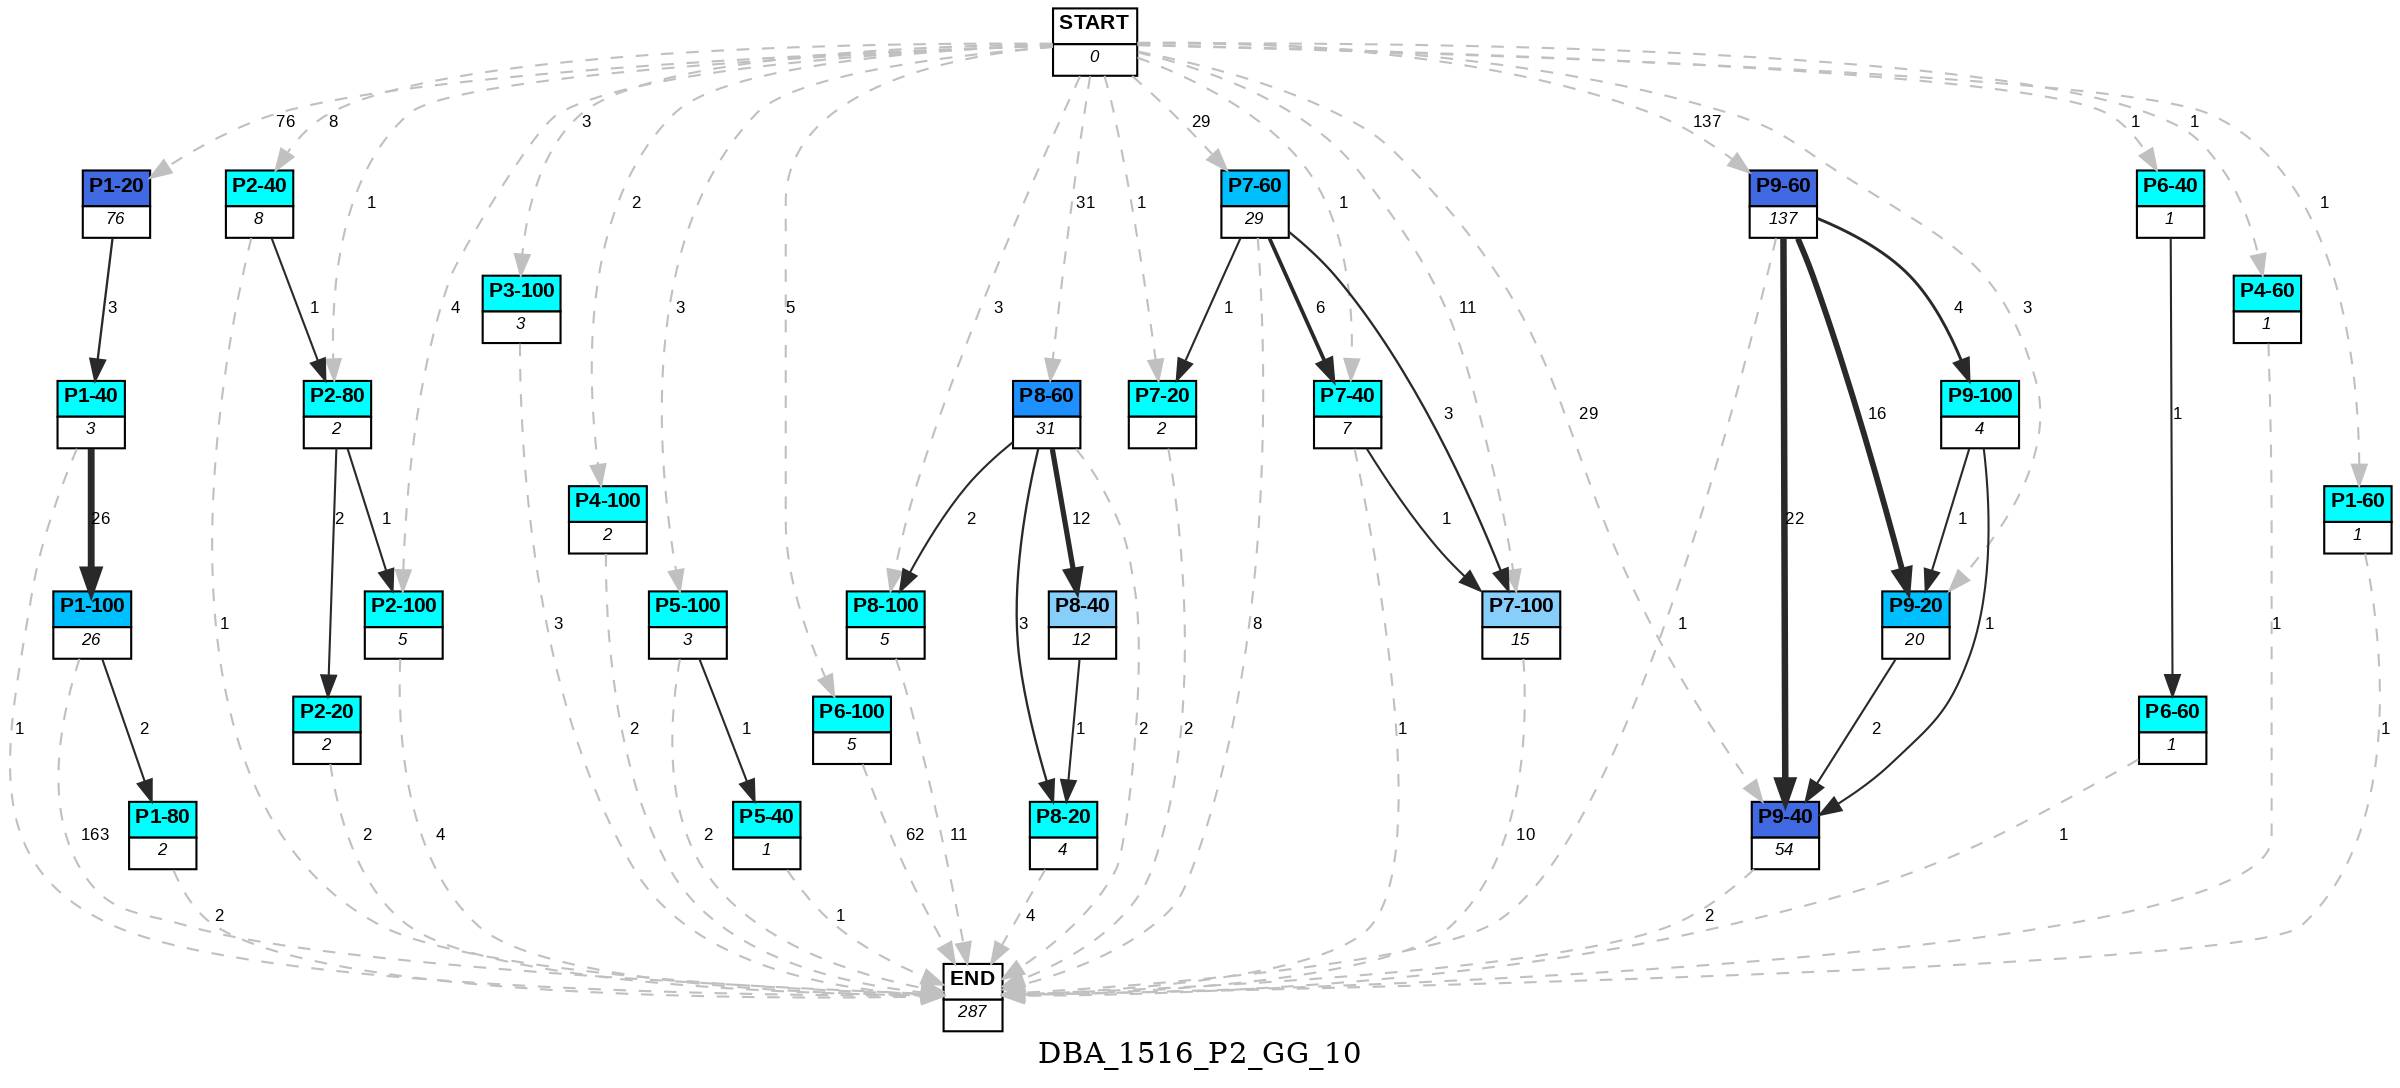
\includegraphics[width=0.4\textwidth]{grafos/DBA_1516_P2_GG_10.png}}\qquad
\subfloat[Grafo que muestra la exploración de los problemas, considerando si un problema ha sido resuelto (\texttt{OK}) o no (\texttt{FAIL}).]{\label{fig:DBA1516P2GG_states}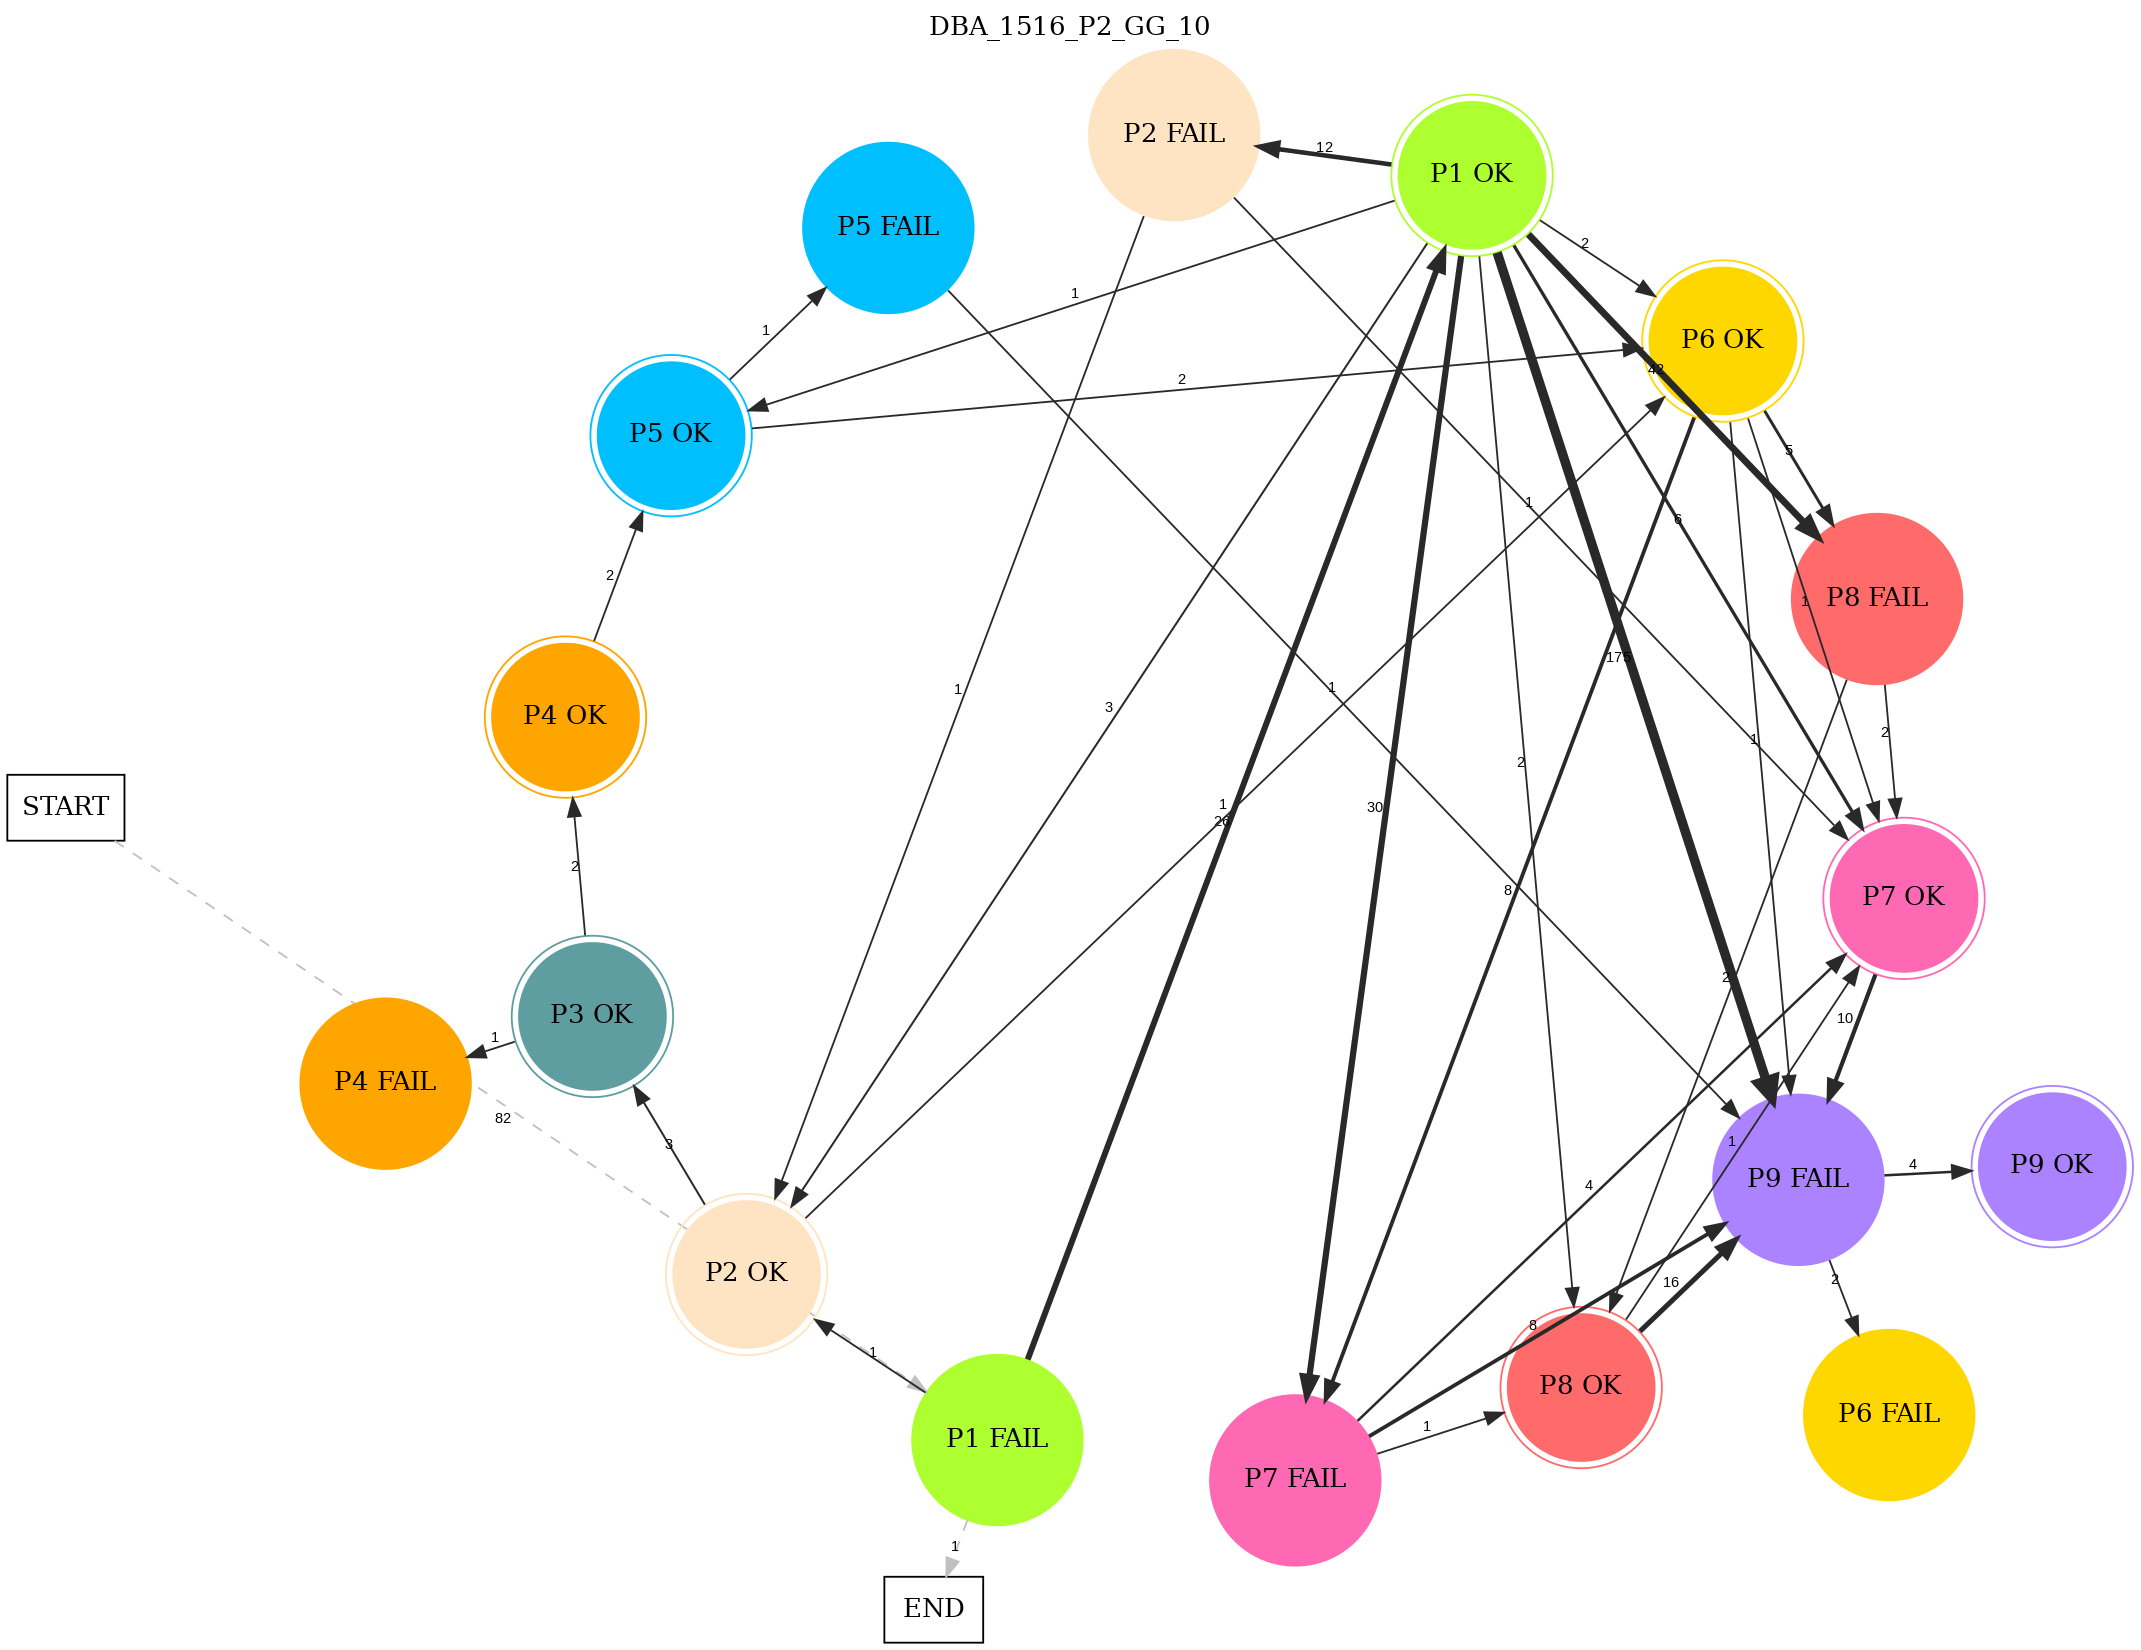
\includegraphics[width=0.7\textwidth]{grafos/DBA_1516_P2_GG_10_wc.png}}
\caption{Leaning Path del grupo de prácticas \texttt{DBA 1516 P2 GG}. Cada nodo se ha coloreado conforme al problema de entre los propuestos que representa. Los valores numéricos que aparecen en cada uno de los enlaces indican la frecuencia con la que se produce cada una de las transiciones. Además, conforme más frecuente sea una conexión mayor será el grosor de la flecha que la representa en el grafo.}
\label{fig:laplacian}
\end{figure}

\subsection{Peso del comportamiento}
Detecta la cantidad de esfuerzo que han dedicado los alumnos a sus tareas de laboratorio en términos del número total de sesiones abiertas en el servidor. Matemáticamente se define como sigue:
\begin{equation}
We(\mathcal{A}) = \sum_r \sum_c \mathcal{A}[r][c]
\end{equation}
\subsection{Eficacia}
Detecta cuantos problemas se han resuelto, simplemente contado el número de nodos $p_k^s$ presentes el grafo. Se formula como sigue:
\begin{equation}
Ef(\mathcal{A}) = \left|\left\lbrace p_i \in P, \sum_r \mathcal{A}[r][p_i^s] > 0 \right\rbrace\right|
\end{equation}
\subsection{Balance}

Trata de determinar cómo de balanceados están los nodos de un grafo dirigido acíclico. De aquí en adelante se denotará por $Ba(\mathcal{A})$.

El coeficiente $Ba$ se calcula a partir de la matriz de adyacencia de un grafo dirigido acíclico. Éste simplemente consiste en calcular la desviación estándar de las componentes de la matriz de adyacencia no nulas y dividirla por la media de dichas entradas.

Todas las métricas generales aquí presentadas se utilizarán para clasificar los grupos de estudiantes. Se ha de tener en cuenta que todas ellas se han definido sobre grafos dirigidos ponderados y no tienen en cuenta absolutamente nada relacionado con el rendimiento de los alumnos ni con los registros temporales de su progreso excepto las funciones $We$ (número de sesiones) y $Ef$ (número de problemas resueltos) y que se extraen únicamente de la matriz característica $\mathcal{A}$.

\begin{figure}[H]
    \centering
    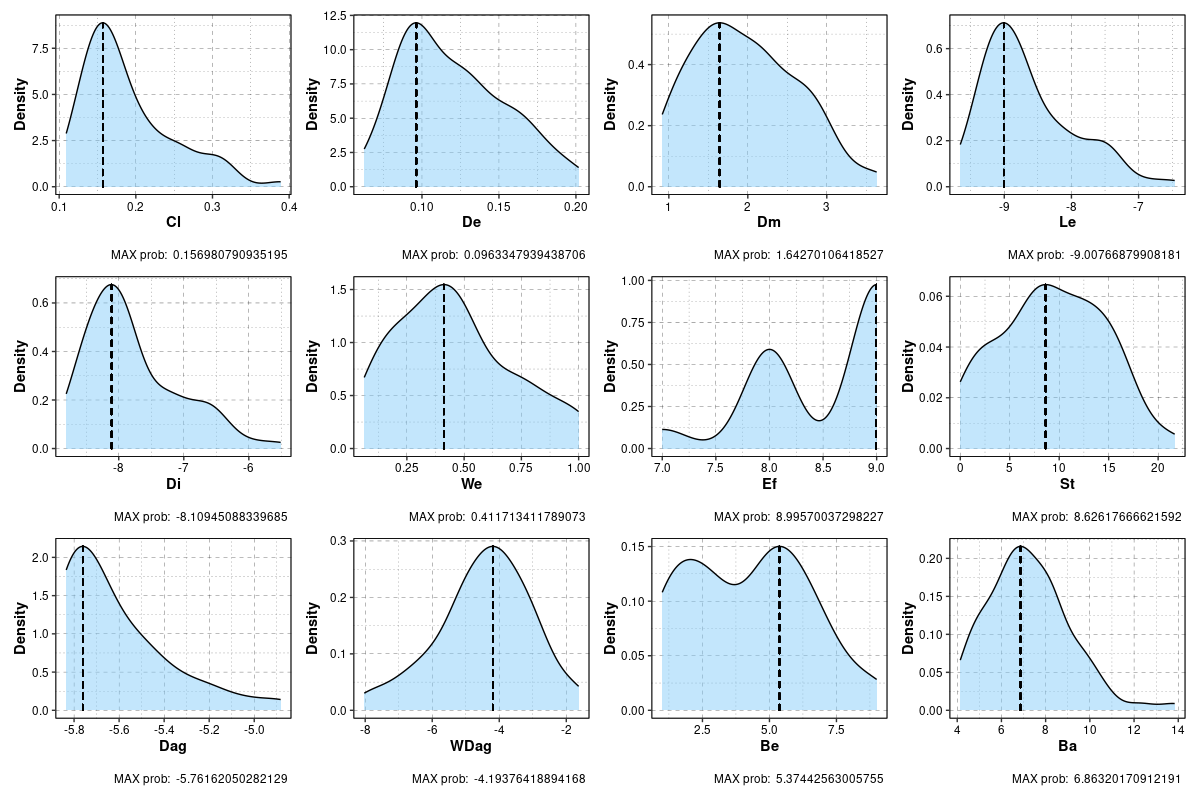
\includegraphics[width=\textwidth]{grafos/densities.png}
    \caption{Funciones de densidad de las métricas topológicas utilizadas en el estudio. Las líneas discontinuas marcan los valores con probabilidad máxima.}
    \label{fig:densities}
\end{figure}

Al tratar con conjuntos de métricas en el análisis estadístico, siempre es un alivio disponer de funciones con distribuciones normales y podemos aceptar que éste es el caso, tal y como se muestra en la Figura \ref{fig:densities}. En dicha imagen podemos ver que, excepto $Ef$ y $Be$, que tienen rangos discretos (número de problemas resueltos y el índice de un problema), todas las métricas restantes podrían considerarse normales, dado el número limitado de grupos que estamos considerando en este estudio. Por otra parte, dado el comportamiento exponencial de algunas de ellas, especialmente las de naturaleza espectral ($Le$, $Di$, $Dag$, $WDag$ y $St$), se han reducido con un logaritmo general con la finalidad de obtener escalas equivalentes en todas las métricas.